\documentclass[12pt]{article}
%THIS IS THE MAIN FILE

% SHARED PREAMBLE START

% THEOREMS, LEMMAS AND COROLLARIES
\usepackage{amsmath}
\usepackage{amssymb}

\newtheorem{theorem}{Theorem}[section]
\newtheorem{corollary}{Corollary}[theorem]
\newtheorem{lemma}[theorem]{Lemma}
\renewcommand\qedsymbol{$\blacksquare$}

%%%%%%%%%%%%%%%%%%%%%%%%%%%%%%%% INKSCAPE
\usepackage{import}
\usepackage{pdfpages}
\usepackage{xifthen}
\usepackage{transparent}
\usepackage{xcolor}
\usepackage[toc,page]{appendix}
\newcommand{\incfig}[2][1]{%
    \def\svgwidth{#1\columnwidth}
    \import{./figures/}{#2.pdf_tex}
}
\pdfsuppresswarningpagegroup=1
%%%%%%%%%%%%%%%%%%%%%%%%%%%%%%%%%%%%%%%%%%%%%%%%
\usepackage[pdftex]{graphicx}
\usepackage{tikz}
\usetikzlibrary{calc}
\usepackage{subfig}
\usepackage{pdfpages}
\usepackage{bm}
%\usepackage{epstopdf}
\usepackage{svg}
\usepackage{hyperref}
\hypersetup{colorlinks=true,
            linkcolor=blue,
            filecolor=magenta,
            urlcolor=cyan,
          }
\usepackage[utf8]{inputenc}
\usepackage[english]{babel}
\usepackage[colorinlistoftodos]{todonotes}
% PAGE FORMATTING
\usepackage{comment}
\usepackage[
backend=biber,
style=alphabetic,
sorting=ynt
]{biblatex}
\addbibresource{../bibliography/Hagedorn.bib}
\addbibresource{../bibliography/Sampling.bib}
\addbibresource{../bibliography/WaveHopping.bib}
\addbibresource{../bibliography/Superadiabatic.bib}

\renewcommand{\baselinestretch}{1.5}

\pagenumbering{roman}

% If LATEX is run on the subfile, the line \documentclass[..]{subfiles} is
% replaced by the preamble of the main file (including its \documentclass
% command). The rest of the subfile is processed normally. If LATEX is run on
% the main file, the subfile is loaded like with an \input command, except that
% the preamble of the subfile up to \begin{document} as well as \end{document}
% and the lines following it are ignored.

% SHARED PREAMBLE END
\numberwithin{equation}{section}

\usepackage{subfiles}


\begin{document}
    
  %%%%%%%%%%%%%%%%%%%%%%%%%%%%%%%%%
  %
  % TABLE OF CONTENTS
  %
  %%%%%%%%%%%%%%%%%%%%%%%%%%%%%%%%%
  \tableofcontents
  % INTRO
  \newpage
\textcolor{blue}{To do:
\begin{itemize}
  \item Background reading: \cite{hagedornRaisingLoweringOperators1998}
  \item Numerics: \cite{faouComputingSemiclassicalQuantum2009} 
  \item Tunneling paper: \cite{gradinaruTunnelingDynamicsSpawning2010}
    - Are they also doing a projection? Or they have an explicit expression 
    for the transition of Hagedorn wavepackets?
  \item Lubich review: \cite{lubichQuantumClassicalMolecular2008} - splitting scheme, 
    hyperbolic cross set, Gaussian quadrature rules
  \item Numerical integration: \cite{bourquinNumericalAlgorithmsSemiclassical2017};
    Gaussian quadrature rules 
  \item Non-adiabatic transitions near avoided crossings: 
    \cite{bourquinNonadiabaticTransitionsAvoided2012} - this is a fully numerical 
    approach, i.e. just extending the Dirac-Frenkel variational 
    approximation. 
  \item Propagation of wavepackets for conical intersections \cite{fermanian-kammererPropagationWavePackets2020}
\end{itemize}}
  %\textbf{Keywords:} complex gaussians; parameter dependent orthonormal basis; 
  %splitting methods; high-dimensional integrals; positive definite (symmetric)
  %\input{intro.tex}
\newpage
    \section{Hagedorn Semiclassical Wavepackets}
      \subfile{hag_intro}
      \subfile{hag_wavepackets} % basis of L2, 
      \subsection{Lowering and Raising operators}
        \begin{itemize}
          \item Eigenvalues and eigenvectors of the d-dimensional 
        Harmonic oscillator
          \item Commutator relations...
          \item This is background reading 
          \item the properties of the raising and lowering operators 
            and then used to derive a recurrence relation for 
        \end{itemize}
        %%%%%%%%%%%%%%%%%%%%%%%%%%%%%%%%%%%%%%%%%%%
        %
        %
        % RECURSIVE RELATION FOR HAGEDORN WAVEPACKETS
        %
        %
        %%%%%%%%%%%%%%%%%%%%%%%%%%%%%%%%%%%%%%%%%%%%
        \subsubsection{Recursive relation for Hagedorn wavepackets}
        For a given parameter set $\Pi$ with matrices 
        $\bm{P}, \bm{Q}$ satisfying Lemma 
        \ref{hagedorn:hagedorn_orthogonal_projection:lemma:symplectic_equations},
        a Schauder orthonormal  
        basis 
        %$\Phi := \{\varphi_k[\Pi]\}_{k \in \mathbb{N}^d}$ 
        for 
        $L^2_{\mathbb{C}} (\mathbb{R}^d, \mathcal{B}(\mathbb{R}^d), \lambda^d)$ 
        can be constructed with the basis vectors 
        $\Phi := \{\varphi_k[\Pi]\}_{k \in \mathbb{N}^d}$ 
        satisfying the following recursive relation 
        \begin{align}
          \varphi_0^{\epsilon} &:= \varphi_0^\epsilon[\Pi](\bm{x})
          \notag
          \\
          \bm{Q} \left(\sqrt{k_j + 1 } \varphi^\epsilon_{k + \langle j \rangle} \right)_{j=1}^d&=
          \sqrt{\frac{2}{\epsilon}} (\bm{x} - \bm{q}) \varphi_k^\epsilon -
          \overline{\bm{Q}}
          \left(\sqrt{k_j} \varphi_{k - \langle j \rangle } \right)_{j=1}^d
          \label{hagedorn:hagedorn_wavepackets:recursive_relation}
        \end{align}
        \textcolor{blue}{Exercise: derive recurrence relation}
        %%%%%%%%%%%%%%%%%%%%%%%%%%%%%%%%%%%%%%%%%%%%%%%%%%%%%%%
        %
        %
        % LATTICE TO SHOWCASE RECURRENCE RELATION 
        %
        %
        %%%%%%%%%%%%%%%%%%%%%%%%%%%%%%%%%%%%%%%%%%%%%%%%%%%%%
        %\subfile{hag_recursionlattice}
      
      \newpage
      \subfile{hag_dynamics} % how to solve things
      \subfile{hag_recursion} 
      \newpage

      \subfile{hag_avoided}
      \subfile{hag_rotation} % needs to be further justified 
      \subfile{hag_projection}  

  \newpage
  \printbibliography
  \begin{appendices}
  \chapter{Some Appendix}
  %\addcontentsline{toc}{chapter}{APPENDICES}
  \section{Transmitted Wavepacket}
  \subfile{hag_transmitted}  
\section{Proof of concept for choosing different parameter set in the 
        projection}
\textcolor{red}{Given that we can obtain the results numerically, 
it is questionable whether this is needed or not}
Here we try to determine/justify whether it is at all 
numerically convenient to change the parameters $\hat{\Pi}$ 
for the transmitted wavepacket and thus reduce the number 
of coefficients needed to represent the wavepacket in the 
Hagedorn basis. This is motivated by the knowledge we have 
regarding the momentum shift.
\\
\\
Since this is only a proof of concept, let us consider the 
simplest complex Gaussian wavepacket for our incoming 
wavepacket with $P = 1, Q = i$. 
Furthermore, we are interested in the dependence of the 
Fourier coefficients with respect to a relative shift $\delta$
in the mean momentum of the transmitted wavepacket and so we 
find it convenient to consider deviations $\delta$ from 
$p = 0$. We also consider the location 
of the avoided crossing to be at $q=0$ 
\textcolor{red}{presumably for the dynamics one can always 
  relocate the avoided crossing to zero by translating the center of mass 
- however this would then now work for on the fly dynamics?}
and thus removing oscillatory terms from the integral.
More precisely we are interested in computing 
$c_k(\delta) = \langle \varphi_0^\epsilon[\delta,0,1,i](\xi),
\varphi_k^\epsilon[0,0,1,i](\xi)  \rangle$. The $\varphi_k$'s 
for this choice of parameters can be generated from the 
recurrence relation
%and let $\tau_k : L^2 \rightarrow L^2$ defined by 
%$f(\xi) \mapsto \tau_k f(\xi) := f(\xi - k)$ denote the 
%translation operator in which case 
%$\tau_k\varphi_0^\epsilon[\hat{\Pi}](\xi) 
%\mapsto \varphi_0^\epsilon[\hat{\Pi}_k](\xi)$, i.e. shifts 
%the momentum from $p$ to $p + k$.
\eqref{hagedorn:hagedorn_wavepackets:recursive_relation}
in momentum space
\textcolor{red}{If I make an ansatz about the polynomial gaussian 
relation, it should give a recurrence relation for the polynomials only}
\textcolor{red}{I would guess that one can do this by first doing the 
translation to $p = 0$ and then re-introducing the translation after 
the tablulation}
\begin{equation}
  \begin{split}
    \varphi_0^\epsilon(\xi) &= 
    (\pi\epsilon)^{-\frac{1}{4}} 
    \exp{\left( - \frac{\xi^2}{2\epsilon} \right)}
    \\
  \varphi^\epsilon_{k + 1} \right)
  &=
  \sqrt{\frac{2}{\epsilon (k + 1)}} \xi \varphi_k^\epsilon -
\sqrt{\frac{k}{k + 1}} \varphi_{k - 1} \right)
  \\
  &= ...
  \\
  &
  \varphi_1^{\epsilon}(\xi) = \sqrt{\frac{2}{\epsilon}}\xi \varphi_0^\epsilon   
  ,\hspace{.5cm}
  \varphi_2^{\epsilon}(\xi) = \left(\sqrt{\frac{2}{\epsilon^2}}\xi^2    
  - \frac{1}{\sqrt{2}}\right)\varphi_0^\epsilon 
  \\
  &
  \varphi_3^{\epsilon}(\xi) = \left(\frac{2}{\sqrt{3\epsilon^3}}\xi^3    
  - \frac{3}{\sqrt{3\epsilon}}\xi \right)\varphi_0^\epsilon 
  ,\hspace{.5cm}
  \varphi_4^{\epsilon}(\xi) = \left(\frac{1}{\epsilon^2}
    \sqrt{\frac{2}{3}}\xi^4    
- \frac{\sqrt{6}}{\epsilon}\xi^2 
 + 
 \sqrt{\frac{3}{8}}\right)\varphi_0^\epsilon 
  \end{split}
\end{equation}
If we let $a_n(\delta) = \langle \varphi_0^\epsilon[\delta,0,1,i](\xi),
  \xi^n \varphi_0^\epsilon[0,0,1,i](\xi)  \rangle$ we can then re-write 
  the coefficients more succintly as
\begin{equation}
  \begin{split}
  &c_1(\delta) = \sqrt{\frac{2}{\epsilon}} a_1(\delta) 
  ,\hspace{0.25cm}
  c_2(\delta) = \sqrt{\frac{2}{\epsilon^2}} a_2(\delta)
  - \frac{1}{\sqrt{2}}a_0(\delta)
  \\
  &c_3(\delta) = \frac{2}{\sqrt{3\epsilon^3}} a_3(\delta)
  - \frac{3}{\sqrt{3\epsilon}} a_1(\delta)
  ,\hspace{0.25cm}
  c_4(\delta) = \frac{1}{\epsilon^2}\sqrt{\frac{2}{3}} a_4(\delta)
  - \frac{\sqrt{6}}{\epsilon}a_2(\delta) + \sqrt{\frac{3}{8}}
  \end{split}
\end{equation}
The polynomials \textcolor{red}{need to check... would they have had 
complex coefficients if we had a complex valued $P$, in higher 
dimension are they linear combinations of monomials or they have 
cross terms?}
are the Hermite polynomials but I still need to get the 
coefficients right...?
Given the form the wavepackets we only need to consider the integral 
for a monomial $\xi^n$ as a prefactor,
\begin{equation}
    \begin{split}
      a_n(\delta) =& (\pi\epsilon)^{-\frac{1}{2}} 
      \int_{\mathbb{R}}
      \xi^n
      \exp{\left[ -\frac{1}{2\epsilon}
      \left(\xi^2 + (\xi - \delta)^2 \right) \right]}
          d\xi
    \\
      =&
      (\pi\epsilon)^{-\frac{1}{2}} 
      \int_{\mathbb{R}}
      \xi^n
      \exp{\left[ -\frac{1}{2\epsilon}
      \left( 2\xi^2 - 2\xi\delta  + \delta^2 \right) \right]}
          d\xi
    \\
      =&
      (\pi\epsilon)^{-\frac{1}{2}} 
      \exp{\left[-\frac{\delta^2}{2\epsilon}\right]}
      \int_{\mathbb{R}}
      \xi^n
      \exp{\left[ -\frac{1}{\epsilon}
      \left( \xi^2 - \xi \delta  \right) \right]}
          d\xi
    \\
      =&
      (\pi\epsilon)^{-\frac{1}{2}} 
      \exp{\left[-\frac{\delta^2}{2\epsilon}\right]}
      \int_{\mathbb{R}}
      \epsilon^n\frac{d^n}{d\delta^n}
      \exp{\left[ -\frac{1}{\epsilon}
      \left( \xi^2 - \xi \delta  \right) \right]}
          d\xi
    \\
      =&
      (\pi\epsilon)^{-\frac{1}{2}} 
      \exp{\left[-\frac{\delta^2}{2\epsilon}\right]}
      \epsilon^n\frac{d^n}{d\delta^n}
      \int_{\mathbb{R}}
      \exp{\left[ -\frac{1}{\epsilon}
      \left( \xi^2 - \xi \delta  \right) \right]}
          d\xi
    \\
      =&
      (\pi\epsilon)^{-\frac{1}{2}} (\pi \epsilon)^{\frac{1}{2}} 
      \epsilon^n
      \exp{\left[-\frac{\delta^2}{2\epsilon}\right]}
    \frac{d^n}{d\delta^n}
    \exp{\left[ \frac{\delta^2}{4\epsilon}  \right]}
    \\
      =&
      \epsilon^n
      \exp{\left[-\frac{\delta^2}{2\epsilon}\right]}
    \frac{d^n}{d\delta^n}
    \exp{\left[-\frac{(i (2\epsilon)^{-\frac{1}{2}}\delta)^2}{2}\right]}
    \\
      =&
      \epsilon^n
      \exp{\left[-\frac{\delta^2}{2\epsilon}\right]}
      \exp{\left[\frac{\delta^2}{4\epsilon}\right]}
      (-i)^n(2\epsilon)^{-n/2}H_n\left(i \frac{\delta}{\sqrt{2\epsilon}}\right) 
    \\
      =&
      \epsilon^n
      \exp{\left[-\frac{\delta^2}{4\epsilon}\right]}
      (-i)^n(2\epsilon)^{-n/2}H_n
      \left(i \frac{\delta}{\sqrt{2\epsilon}}\right) 
    \end{cases}
     \end{split}
  \end{equation}
  where we have used the a known identity for the Gaussian integral and the 
  probabilists' Hermite polynomials $H_e(x)= ...$
  %\cite{hermiteOEuvresCharlesHermite1864}.
  \begin{itemize}
    \item $a_0(\delta) = c_0(\delta)$
    \item $a_0(0) = c_0(0) = 1$ as expected
    \item Checked the first few but the following plot 
      will also serve as a sanity check
    \item This makes clearer Hagedorn and Joye's claim that the 
      leading order is a Gaussian 
    \item If we consider the $c_n$'s it does seem as if 
      the dependence on the higher order basis vectors is in ascending 
      order as we increase $\delta$ up to a certain point
    \item It is intuitively clear why it depends on the ratio between the
      momentum shift and the variance $\mathcal{O}(\epsilon)$
    \item The coefficients are real because we have chosen $q=0$
    \item We know that the mean momentum shift is at least $2\sqrt{\delta}$
      from conservation of energy 
  \end{itemize}
  \begin{figure}[h!]
  % GNUPLOT: LaTeX picture with Postscript
\begingroup
  \makeatletter
  \providecommand\color[2][]{%
    \GenericError{(gnuplot) \space\space\space\@spaces}{%
      Package color not loaded in conjunction with
      terminal option `colourtext'%
    }{See the gnuplot documentation for explanation.%
    }{Either use 'blacktext' in gnuplot or load the package
      color.sty in LaTeX.}%
    \renewcommand\color[2][]{}%
  }%
  \providecommand\includegraphics[2][]{%
    \GenericError{(gnuplot) \space\space\space\@spaces}{%
      Package graphicx or graphics not loaded%
    }{See the gnuplot documentation for explanation.%
    }{The gnuplot epslatex terminal needs graphicx.sty or graphics.sty.}%
    \renewcommand\includegraphics[2][]{}%
  }%
  \providecommand\rotatebox[2]{#2}%
  \@ifundefined{ifGPcolor}{%
    \newif\ifGPcolor
    \GPcolortrue
  }{}%
  \@ifundefined{ifGPblacktext}{%
    \newif\ifGPblacktext
    \GPblacktexttrue
  }{}%
  % define a \g@addto@macro without @ in the name:
  \let\gplgaddtomacro\g@addto@macro
  % define empty templates for all commands taking text:
  \gdef\gplbacktext{}%
  \gdef\gplfronttext{}%
  \makeatother
  \ifGPblacktext
    % no textcolor at all
    \def\colorrgb#1{}%
    \def\colorgray#1{}%
  \else
    % gray or color?
    \ifGPcolor
      \def\colorrgb#1{\color[rgb]{#1}}%
      \def\colorgray#1{\color[gray]{#1}}%
      \expandafter\def\csname LTw\endcsname{\color{white}}%
      \expandafter\def\csname LTb\endcsname{\color{black}}%
      \expandafter\def\csname LTa\endcsname{\color{black}}%
      \expandafter\def\csname LT0\endcsname{\color[rgb]{1,0,0}}%
      \expandafter\def\csname LT1\endcsname{\color[rgb]{0,1,0}}%
      \expandafter\def\csname LT2\endcsname{\color[rgb]{0,0,1}}%
      \expandafter\def\csname LT3\endcsname{\color[rgb]{1,0,1}}%
      \expandafter\def\csname LT4\endcsname{\color[rgb]{0,1,1}}%
      \expandafter\def\csname LT5\endcsname{\color[rgb]{1,1,0}}%
      \expandafter\def\csname LT6\endcsname{\color[rgb]{0,0,0}}%
      \expandafter\def\csname LT7\endcsname{\color[rgb]{1,0.3,0}}%
      \expandafter\def\csname LT8\endcsname{\color[rgb]{0.5,0.5,0.5}}%
    \else
      % gray
      \def\colorrgb#1{\color{black}}%
      \def\colorgray#1{\color[gray]{#1}}%
      \expandafter\def\csname LTw\endcsname{\color{white}}%
      \expandafter\def\csname LTb\endcsname{\color{black}}%
      \expandafter\def\csname LTa\endcsname{\color{black}}%
      \expandafter\def\csname LT0\endcsname{\color{black}}%
      \expandafter\def\csname LT1\endcsname{\color{black}}%
      \expandafter\def\csname LT2\endcsname{\color{black}}%
      \expandafter\def\csname LT3\endcsname{\color{black}}%
      \expandafter\def\csname LT4\endcsname{\color{black}}%
      \expandafter\def\csname LT5\endcsname{\color{black}}%
      \expandafter\def\csname LT6\endcsname{\color{black}}%
      \expandafter\def\csname LT7\endcsname{\color{black}}%
      \expandafter\def\csname LT8\endcsname{\color{black}}%
    \fi
  \fi
    \setlength{\unitlength}{0.0500bp}%
    \ifx\gptboxheight\undefined%
      \newlength{\gptboxheight}%
      \newlength{\gptboxwidth}%
      \newsavebox{\gptboxtext}%
    \fi%
    \setlength{\fboxrule}{0.5pt}%
    \setlength{\fboxsep}{1pt}%
\begin{picture}(7200.00,4320.00)%
    \gplgaddtomacro\gplbacktext{%
      \csname LTb\endcsname%%
      \put(645,595){\makebox(0,0)[r]{\strut{}$0$}}%
      \csname LTb\endcsname%%
      \put(645,1228){\makebox(0,0)[r]{\strut{}$0.2$}}%
      \csname LTb\endcsname%%
      \put(645,1861){\makebox(0,0)[r]{\strut{}$0.4$}}%
      \csname LTb\endcsname%%
      \put(645,2495){\makebox(0,0)[r]{\strut{}$0.6$}}%
      \csname LTb\endcsname%%
      \put(645,3128){\makebox(0,0)[r]{\strut{}$0.8$}}%
      \csname LTb\endcsname%%
      \put(645,3761){\makebox(0,0)[r]{\strut{}$1$}}%
      \csname LTb\endcsname%%
      \put(747,409){\makebox(0,0){\strut{}$0$}}%
      \csname LTb\endcsname%%
      \put(1976,409){\makebox(0,0){\strut{}$0.2$}}%
      \csname LTb\endcsname%%
      \put(3205,409){\makebox(0,0){\strut{}$0.4$}}%
      \csname LTb\endcsname%%
      \put(4435,409){\makebox(0,0){\strut{}$0.6$}}%
      \csname LTb\endcsname%%
      \put(5664,409){\makebox(0,0){\strut{}$0.8$}}%
      \csname LTb\endcsname%%
      \put(6893,409){\makebox(0,0){\strut{}$1$}}%
    }%
    \gplgaddtomacro\gplfronttext{%
      \csname LTb\endcsname%%
      \put(153,2178){\rotatebox{-270}{\makebox(0,0){\strut{}$|c_k|$}}}%
      \csname LTb\endcsname%%
      \put(3820,130){\makebox(0,0){\strut{}$\delta$}}%
      \csname LTb\endcsname%%
      \put(3820,4040){\makebox(0,0){\strut{}$\epsilon = 0.05$}}%
      \csname LTb\endcsname%%
      \put(6105,3594){\makebox(0,0)[r]{\strut{}$k=0$}}%
      \csname LTb\endcsname%%
      \put(6105,3408){\makebox(0,0)[r]{\strut{}$k=1$}}%
      \csname LTb\endcsname%%
      \put(6105,3222){\makebox(0,0)[r]{\strut{}$k=2$}}%
      \csname LTb\endcsname%%
      \put(6105,3036){\makebox(0,0)[r]{\strut{}$k=3$}}%
    }%
    \gplbacktext
    \put(0,0){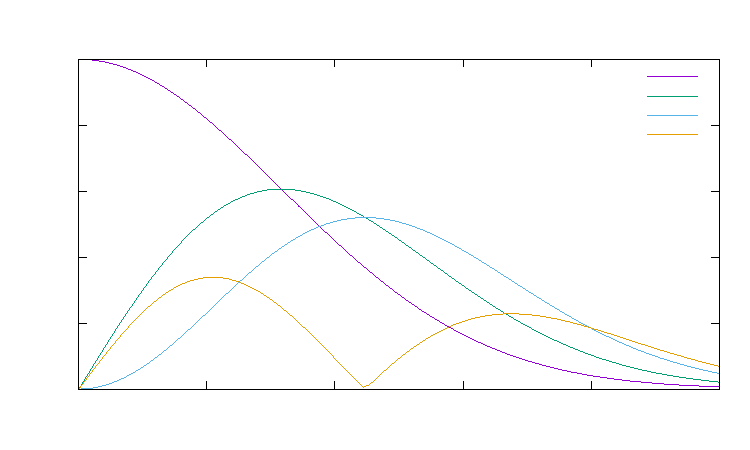
\includegraphics{plots/hagedorn_coeff}}%
    \gplfronttext
  \end{picture}%
\endgroup

  \caption{$c_k$ is the coefficient corresponding to the projected Gaussian 
  onto the $k^{\text{th}}$ Hagedorn wavepacket.}
  \end{figure}
\subsection{One dimensional case}
(Ignore global phase factor for the moment)
In one dimension the $a_{kl}$ becomes 
\begin{equation}
  \begin{split}
    a_{kl} &= 
    \sin\left(\frac{\pi \gamma}{2}\right)
    \int_{\mathbb{R}} \text{sgn}(\xi_1) \Theta(\xi_1^2 - 4\delta)
    \left( 1 + \frac{\xi_1}{\nu(\xi_1)} \right)
      P_k[\hat{\Pi}^{\pm}_{t_c}](\tilde{\xi})
      \overline{ P_l[\hat{\Pi}^\prime](\xi)} 
    \times 
    \\
    &
    \hspace{1cm}
    \exp \Bigg[-\frac{1}{2\epsilon} 
        \Big( \alpha (\nu(\xi_1) - p_1)^2 + \overline{\alpha} (\xi_1 - p_1^\prime)^2
          + \beta (\nu(\xi_1) - p_1) + \overline{\beta} (\xi_1 - p_1^\prime)
    \\
    &
    \hspace{1cm}
    + 2q_c|\xi_1 - \nu(\xi_1)|
      \Big) 
    \Bigg]  d \xi_1 
    \\
  \end{split}
\end{equation}
where 
\begin{equation}
  \begin{split}
  \alpha = I_{11} - i R_{11} &\hspace{1cm}  
    \beta = -i2q_1 
  \end{split}
\end{equation}
and (see attached written notes)
\begin{equation}
  \begin{split}
  P_{k}[\Pi](x) \varphi_0&= 
  \sqrt{k!} \left( \frac{i}{2\epsilon} \right)^k
  \sum_{\substack{j=0 \\ j \equiv k (\text{mod} 2)}}^k \frac{(i \epsilon Q^*P^*/2)^{(k-j)/2}}{j! (\frac{k-j}{2})!}
  \times
  \\
  &\times 
  \left(
    \sum_{r=0}^j \binom{j}{r} \left( P^*(x-q) + Q^*p  \right)^r
    \left( Q^*i\epsilon d_x  \right)^{j - r}
  \right)
  \varphi_0
  \end{split}
\end{equation}
so that 
\begin{equation}
  \begin{split}
  P_{k}[\Pi](x) &= 
  \sqrt{k!} \left( \frac{i}{2\epsilon} \right)^k
  \sum_{\substack{j=0 \\ j \equiv k (\text{mod} 2)}}^k \frac{(i \epsilon Q^*P^*/2)^{(k-j)/2}}{j! (\frac{k-j}{2})!}
  \times
  \\
  &\times 
  \Bigg(
    \sum_{r=0}^j \binom{j}{r} \left( P^*(x-q) + Q^*p  \right)^r
    \left( Q^* i \epsilon \right)^{j-r}
    \sum_{l=0}^{\lfloor{j-r}\rfloor}\sum_{s=0}^{j - r - 2l}
    \binom{j-r-2l}{s} 
  \\
  &\times
    \left( i\epsilon PQ^{-1}(x - q)  \right)^{j - r -2l -s}
    \left( \frac{i}{\epsilon} p   \right)^s
    \left( i \epsilon PQ^{-1}   \right)^l \frac{(j-r)!}{l!(j - r - 2l)!}2^{-l}
  \Bigg)
  \end{split}
\end{equation}
\\
\begin{itemize}
  \item there is an extra parity condition on $j$ which you are missing
  \item Polynomial has degree $k$ and so we would need 
    at most $k + 1$ terms in the summation. So how can we go about 
    simplifying the expression further, perhaphs using properties 
    of $P,Q$ from Lemma 1.1 and a bit of manipulation
  \item The expression can most likely be simplified further - for 
    the moment we will just going to use it to see if it is at least 
    correct
  \item verify expression reduces to 
    Hermite polynomial for particular parameter values
  \item Plot result from expression against one from 
    recurrence relation 
  \item Start by considering $k = 0$ for ease so only one subsitution
  \item You should be able to evaluate the second term recursively
\end{itemize}
Before attempting any simplification we will start by considering the $a_{0l}$'s with
$\hat{\Pi}^\prime = \{P = 1, Q = i, q=0, p=p^\prime\}$ 
for which
\\
\textbf{Example}
\\
\textcolor{red}{In certain sense we can already comment on the 
dependence of the ... based on the proof concept in one of previous 
sections}
\begin{equation}
  \begin{split}
    P_{l}[\hat{\Pi}^\prime](\xi) &= 
    \sqrt{k!} \left( \frac{i}{2\epsilon} \right)^k
    \sum_{\substack{j=0 \\ j \equiv k (\text{mod} 2)}}^k \frac{(\epsilon/2)^{(k-j)/2}}{j! (\frac{k-j}{2})!}
    \times
      \sum_{r=0}^j \binom{j}{r} 
      \epsilon^j
      i^j\left( -\frac{1}{\epsilon}(\xi-p^\prime) \right)^r
    \\
    &\times 
    \Bigg(
    \sum_{l=0}^{\lfloor{j-r}\rfloor}
    \left(-\frac{1}{\epsilon}(\xi - p^\prime)
    \right)^{j - r -2l}\left( -\frac{1}{\epsilon}\right)^l
    2^{-l}\frac{(j-r)!}{l!(j - r -2l)!}
  \Bigg)
  \\
    &
    = \sqrt{k!} \left( \frac{1}{2\epsilon} \right)^k
    \sum_{\substack{j=0 \\ j \equiv k (\text{mod} 2)}}^k \frac{(\epsilon/2)^{(k-j)/2}}{(\frac{k-j}{2})!}
      \epsilon^j
      i^{j + k}
    \times
    \sum_{r=0}^j \frac{1}{r!} 
    \\
    &\times 
    \sum_{l=0}^{\lfloor{j-r}\rfloor}
    (-2\epsilon)^{-l}\frac{1}{l!(j - r -2l)!}
    \left(-\frac{1}{\epsilon}(\xi - p^\prime)
    \right)^{j -2l}
  \end{split}
\end{equation}
Perhaps it is easier to consider the cases where $k$ is 
even or odd
\\
The $i$ dependence cancels since $k,j$ have the same parity 
\\
\\
since this should reduce to the expression for the Hermite 
polynomials except some $\epsilon$
With regards to the integral, let us first consider the case $k=0$
\begin{equation}
  \begin{split}
    a_{0l} &=  
    \int_{\mathbb{R}} \text{sgn}(\xi_1) \Theta(\xi_1^2 - 4\delta)\left( 1 + \frac{\xi_1}{\nu(\xi_1)} \right)
      \overline{ P_l[\hat{\Pi}^\prime](\xi)} 
    \times 
    \\
    &
    \hspace{1cm}
    \exp \Bigg[-\frac{1}{2\epsilon} 
        \Big( (\nu(\xi_1) - p_1)^2 + (\xi_1 - p_1^\prime)^2
    + 2q_c|\xi_1 - \nu(\xi_1)|
      \Big) 
    \Bigg]  d \xi_1 
    \\
  \end{split}
\end{equation}
\textcolor{red}{As we have argued the polynomials will be real valued in this case.}
\\
If we Taylor expand $\tilde{a}_1 = \nu(\xi_1) - p_1$ about $p_1^\prime$ to first order we have,
\begin{equation}
  \begin{split}
    \tilde{a}_1 &= \text{sgn}(\xi_1)\sqrt{\xi_1^2 - 4\delta} - p_1
  =
  \text{sgn}(\xi_1) \sum_{n=0} ...
  \\
  &
  = \text{sgn}(\xi_1) \left( \sqrt{p_1^\prime^2 - 4\delta} - p_1 + 
    \frac{p_1^\prime}{\sqrt{p_1^\prime^2 - 4\delta}} (\xi - p_1^\prime) 
  + ...
  \right)
  \end{split}
  \notag
\end{equation}
i.e. of the form $\alpha + \beta(\xi_1 - p_1^\prime)$
\textcolor{red}{the remainder can also be formulated as an integral - which one is most convenient}
and assume the wavepacket's momentum is large and positive .
Further, with expanding $\nu(\xi_1)$ using the binomial theorem 
\begin{equation}
  \begin{split}
  \nu(\xi_1) &= \text{sgn}(\xi_1)\sqrt{\xi_1^2 - 4\delta}
  =
  \xi_1\sqrt{1 - \frac{4\delta}{\xi_1^2}}
  = \xi_1 \sum_{n=0}^{\infty} ...
  \\
  &=
\xi_1 (1 - \frac{2\delta}{\xi_1^2} - \frac{2\delta^2}{\xi_1^4} + ...)
= \xi_1 - \frac{2\delta}{\xi_1} - \frac{2\delta^2}{\xi_1^3} + ...
  \end{split}
  \notag
\end{equation}
yields - ``contribution to integral comes from positive axis" -
\textcolor{red}{is the integration known over half domain}
\begin{equation}
  \begin{split}
    a_{0l} &\approx 
    2 \exp{\left[
        -\frac{1}{2\epsilon} (\alpha^2 + p_1^\prime - p_1 - \alpha) 
    \right]}
    \int_{\mathbb{R}} 
    \overline{ P_l[\hat{\Pi}^\prime](\xi)} 
    \times 
    \\
    &
    \hspace{1cm}
    \exp \Bigg[-\frac{1}{2\epsilon} 
      \Big( (\beta^2 + 1)(\xi_1 - p_1^\prime)^2
        +
        (2\alpha \beta + \beta + 1) (\xi_1 - p_1^\prime)
      \Big) 
    \Bigg]  d \xi_1 
    \\
    & =  
    2 \exp{\left[
        -\frac{1}{2\epsilon} (\alpha^2 + p_1^\prime - p_1 - \alpha) 
    \right]}
    \int_{\mathbb{R}} 
    \overline{ P_l[\hat{\Pi}^\prime](u + p_1^\prime)} 
    \times 
    \\
    &
    \hspace{1cm}
    \exp \Bigg[-\frac{1}{2\epsilon} 
      \Big( \gamma u^2
        +
        \zeta u
      \Big) 
    \Bigg]  d u 
    \\
    & =  
    2 \exp{\left[
        -\frac{1}{2\epsilon} (\alpha^2 + p_1^\prime - p_1 - \alpha) 
    \right]}
   \sqrt{k!} \left( \frac{1}{2\epsilon} \right)^k
    \sum_{\substack{j=0 \\ j \equiv k (\text{mod} 2)}}^k \frac{(\epsilon/2)^{(k-j)/2}}{(\frac{k-j}{2})!}
      \epsilon^j
      i^{j + k}
    \times
    \sum_{r=0}^j \frac{1}{r!} 
    \\
    &\times 
    \sum_{l=0}^{\lfloor{j-r}\rfloor}
    (-2\epsilon)^{-l}\frac{1}{l!(j - r -2l)!}
    \left(-\frac{1}{\epsilon}
    \right)^{j -2l}
    \int_{\mathbb{R}} 
    u^{j - 2l}
    \exp \Bigg[-\frac{1}{2\epsilon} 
      \Big( \gamma u^2
        +
        \zeta u
      \Big) 
    \Bigg]  d u 
    \\
  \end{split}
\end{equation}
The integral above can be solved as 
\begin{equation}
  \begin{split}
    &\int_{\mathbb{R}} 
    -(2\epsilon)^{j-2l}
    \frac{d^{j-2l}}{d\zeta}
    \exp \Bigg[-\frac{1}{2\epsilon} 
      \Big( \gamma u^2
        +
        \zeta u
      \Big) 
    \Bigg]  d u 
    \\
    &=
    -(2\epsilon)^{j-2l}
    \frac{d^{j-2l}}{d\zeta}
    \int_{\mathbb{R}} 
    \exp \Bigg[-\frac{1}{2\epsilon} 
      \Big( \gamma u^2
        +
        \zeta u
      \Big) 
    \Bigg]  d u 
    \\
    &=
    -(2\epsilon)^{j-2l}
    \sqrt{\frac{\pi}{\gamma}} 
    \frac{d^{j-2l}}{d\zeta}
    \exp{\left[
      \frac{\zeta^2}{4\gamma}
    \right]}
  \end{split}
\end{equation}
and the derivatives once again give rise to Hermite 
polynomials
\\
I still need to get round to test it 
%\\
%Plot $\sqrt{\xi^2 - 4\delta}$ against its linear 1st order approximation - to see how good it is
\\
\textcolor{red}{I can always consider smoothing the cut-off function with a bump function and take the 
limit outside...?}
%
\newpage
\textbf{Change of variables --> Asymptotic expansion via stationary phase principle}
This would work only in 1d as there is no stationary point in d>1
\\
\textbf{Changing range of integration}
\\
Consider 
\begin{equation}
  \begin{split}
    \int_{2\sqrt{\delta}}^\infty f(\xi) \exp{\left[-\frac{i}{2\epsilon} ()  \right]} d\xi
  \end{split}
\end{equation}
\\
\section{Transmitted wavepacket recurrence relation derivation}
We have
\begin{equation}
  \begin{split}
    &\Big(
      \langle 
      (\tilde{\bm{\xi}}-\bm{q})_j^p 
      f(\tilde{\bm{\xi}})
      \tilde{\varphi}_{k + \langle j \rangle},
    \varphi_l \rangle
  \Big)_{j=1}^d
    =
    \\
      =&
    \Big(
      \sum_{i=1}^d
     \bm{A}_{j,i} 
     \langle (\tilde{\bm{\xi}}-\bm{q})^p_j
     (\tilde{\bm{\xi}}-\bm{q})_{i}
      f(\tilde{\bm{\xi}})
      \tilde{\varphi_k}, 
      \varphi_l \rangle
    \Big)_{j=1}^d
    - \Big(
      \sum_{i=1}^d
      \bm{B}_{j,i}
      \langle 
      (\tilde{\bm{\xi}}-\bm{q})_j^p
      f(\tilde{\bm{\xi}})
      \tilde{\varphi}_{k - \langle i  \rangle}
      , \varphi_l \rangle
      \Big)_{j=1}^d
  \end{split}
\end{equation}
and then proceeding in a similar manner as before 
for the higher order cross terms. 
Now, let $k$ be fixed and $l$ vary giving 
\begin{equation}
  \begin{split}
    &\Big(
      \langle 
      f(\tilde{\bm{\xi}})
      \tilde{\varphi}_{k },
    (\bm{\xi}-\bm{q})_j^p 
    \varphi_{l+ \langle j \rangle}  \rangle
  \Big)_{j=1}^d
    =
    \\
      =&
    \Big(
      \sum_{i=1}^d
     \bm{A}_{j,i} 
     \langle 
      f(\tilde{\bm{\xi}})
      \tilde{\varphi_k}, 
     (\bm{\xi}-\bm{q})^p_j
     (\bm{\xi}-\bm{q})_{i}
      \varphi_l \rangle
    \Big)_{j=1}^d
    - \Big(
      \sum_{i=1}^d
      \bm{B}_{j,i}
      \langle 
      f(\tilde{\bm{\xi}})
      \tilde{\varphi}_{k}
      ,
      (
      \bm{\xi}-\bm{q})_j^p
      \varphi_{l- \langle i  \rangle} 
      \rangle
      \Big)_{j=1}^d
  \end{split}
\end{equation}
and then for the higher moments similarly.

\end{appendices}

\end{document}

